\section{The margin read by a learned score: two dimensions}
\label{sec:twodim}

\begin{figure*}[t]
\centering
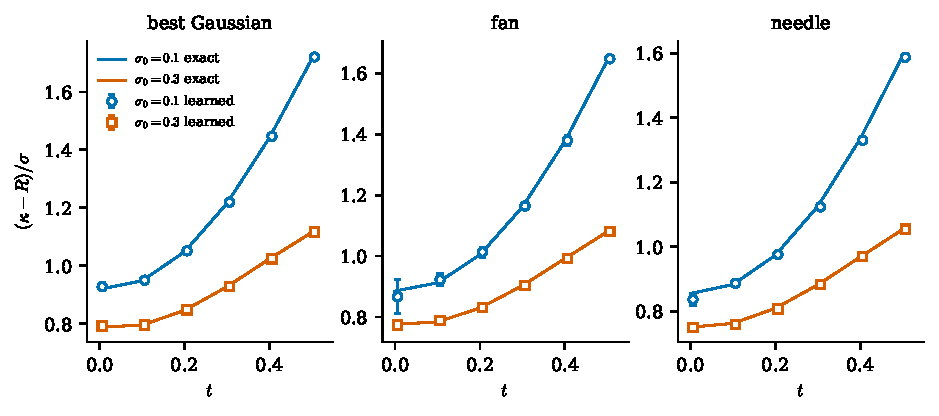
\includegraphics[width=0.9\textwidth]{figures/fig2_learned_2d.pdf}
\caption{Pendulum: the margin $(\kappa - R)/\sigma$ read from learned networks (symbols, with error band) against the exact value (lines), for $0 \leq t \leq 0.5$ at $r = 1$. Left to right: best Gaussian state, fan, needle. Circles: $\sigma_0 = 0.1$; squares: $\sigma_0 = 0.3$.}
\label{fig:learned2d}
\end{figure*}

\begin{observation}
\label{obs:2d}
For the three states and $\sigma_0 = 0.1$, $0.3$, the margin read from the learned networks with the divergence form agrees with the exact margin to within $2.15\%$ at all 36 points ($t = 0, 0.1, \dots, 0.5$). At 32 of them the difference lies inside the error band.
\end{observation}

Figure~\ref{fig:learned2d} shows the comparison. At $t = 0$ and $\sigma_0 = 0.1$ the distance $\kappa - R$ is only $8$--$9\%$ of $\kappa$, and the learned score resolves it with an error of at most about $2\%$ of itself, that is, $0.2\%$ of $R$. The two largest differences are at $t = 0$ and $\sigma_0 = 0.1$, for the fan ($-2.09\%$, inside a wide band) and for the needle ($-2.15\%$, outside its band). These are the sharpest states: their learned scores have $\eta_s = 0.013$ and $0.020$, above the $10\%$ target of Table~\ref{tab:required}, while for the best Gaussian state $\eta_s = 0.003$--$0.006$ and the differences stay below $1\%$. The other two points outside the band differ by $0.4$--$0.5\%$, where the band is narrow. As $t$ grows the state leaves the top, the margin grows, and the relative difference shrinks.

The form of the estimator is decisive. With the plain form~\eqref{eq:Rplain}, the same networks miss the margin of the best Gaussian state at $\sigma_0 = 0.1$, $t = 0$ by $14\%$; with the divergence form the miss is $1\%$.

\emph{The limit of our networks.} At $\sigma_0 = 0.03$ the required accuracy is $\eta < 0.003$ (Table~\ref{tab:required}). With batch size 16384 the learned score reached $\eta_s = 0.0018$--$0.0029$ for $0.1 \leq t \leq 0.5$, and the margin agreed with the exact one to within $0.7\%$ there, but at $t = 0$ it stayed at $\eta_s = 0.0036$, with a difference of $-2.1\%$. Increasing the batch size from 4096 to 16384 did not lower the error at $t = 0$, so gradient noise is no longer the limit there. We report $\sigma_0 = 0.03$ as a reference only and do not include it in the claims.
